\documentclass[a4paper]{jpconf}
\bibliographystyle{iopart-num}
\usepackage{amsmath}
\usepackage{citesort}
\usepackage{subfigure}
\usepackage{graphicx}
\graphicspath{{fig/}}
\usepackage{ifpdf}
\ifpdf\usepackage{epstopdf}\fi
\usepackage[export]{adjustbox}

%----------------------------------------------------- 
%\usepackage{soul,ulem,color,xspace,bm}
% Andrei's commands
% Suggest to remove
%\newcommand{\asrm}[1]{{\color{magenta}\sout{#1}}}
% Suggest to insert
%\newcommand{\as}[1]{\color{cyan}#1\xspace\color{black}}
% Suggest to replace
%\newcommand{\asrp}[2]{\asrm{#1} \as{#2}}
% Comment
%\newcommand{\ascm}[1]{{\color{green}\;AS: #1}}
%------------------------------------------------------

\begin{document}
\title{Particle-in-cell simulation of shock waves with different kinds of ions.}

\author{V I Romanky$^{1,2}$, A M Bykov$^1$, S M Osipov$^1$ and P E Gladilin$^1$}

\address{$^1$ Ioffe Institute, 26 Politekhnicheskaya st., St. Petersburg 194021, Russia}
\address{$^2$ 
Sternberg Astronomical Institute, Moscow State University
 Universitetsky pr., 13, Moscow 119234, Russia}

\ead{romanskyvadim@gmail.com}

\begin{abstract}
The problem of Cosmic Ray (CR) origin and acceleration is a widely discussed problem of
modern astrophysics. It is considered that most likely CR sources are supernova remnant
shock waves. One of the methods to study particle injection and acceleration by shock
waves is a particle-in-cell computer simulation. In this paper we present results of shock
wave simulations based on our self-developed implicit particle-in-cell code. First, we test the code
with the well-known two stream and Weibel instabilities and second, simulate shock waves in
plasma with different particle composition. Using the obtained results we study the
process of charged particle acceleration at the shock front.
\end{abstract}
\section{Introduction}
One of the possible sources of high-energy cosmic rays are shock waves in astrophysical collisionless plasma due to the diffusive shock acceleration (DSA) mechanism, see \cite{Bell1978}, \cite{Blandford1978}. Strong magnetic fields are necessary for effective acceleration of charged particles and the observations of the synchrotron emission from supernova remnants (SNRs) show, that the magnetic field there is about 100 times stronger then the interstellar field (see for example \cite{Berezhko2003},\cite{Uchiyama2007}). So strong fields can be produced due to instabilities in anisotropic plasma. One of the most powerful methods to explore processes in collisionless plasma is the Particle-in-Cell simulation. In this work we explore instabilities in the plasma using this method. 
We developed the implicit particle-in-cell (PIC) code, based on the scheme suggested by Lapenta et al.~\cite{Lapenta2006} and improved for the relativistic case by Noguchi et al.\cite{Noguchi2007}.
Our code is fully three dimensional and parallelized with MPI technology, which is adapted for distributed computing and can be executed on a wide class of computers.
\section{Model of implicit particle-in-cell}
We developed the implicit particle-in-cell (PIC) code, based on the scheme suggested by Lapenta et al.~\cite{Lapenta2006} and improved for the relativistic case by Noguchi et al.\cite{Noguchi2007}. This scheme is described in details in these papers and below we present only a short description. The common assumption for all particle-in-cell codes is the consideration of the plasma as a superposition of a large number of finite elements, called super-particles. Distribution function can be represented as the sum of members for all super-particles: 
\begin{equation}
F \left( \textbf{x},\textbf{p},t \right) =\sum _{p=1}^{N_{s}}S \left( x-x_{{p}} \right) 
S \left( y-y_{{p}} \right) S \left( z-z_{{p}} \right) \delta \left( \textbf{p}-\textbf{p}_{{p}} \right), 
\end{equation}
where $\textbf{x}$ and $\textbf{p}$ are coordinates and the momentum of a particle , respectively, $S$ is a shape-function, and $\delta$ is the Dirac's delta-function. The shape-function is chosen in form of b spline. Also we introduce interpolation function $W$ which represents the part of a particle which is contained in the grid cell:
\begin{equation}
W \left(x_{{c}} - x_{{p}} \right)= \int\limits_{-\infty}^{+\infty}S(x-x_{{p}})\phi(x)dx,
\end{equation} 
where $c$ and $p$ are indexes of the cell and the particle, respectively, and $\phi$ equals 1 inside the cell and 0 outside. Using this function we can determine electric and magnetic field for each particle as
\begin{equation}
\begin{aligned}
&\textbf{E}_{p} = \sum_{c}\textbf{E}_c W \left(x_{{c}} - x_{{p}} \right),
\\
&\textbf{B}_{p} = \sum_{c}\textbf{B}_c W \left(x_{{c}} - x_{{p}} \right).
\end{aligned}
\end{equation}

Then we use particle fields to solve equations of motion for particles:
\begin{equation}
\begin{aligned}
&{\frac {d\textbf{x}_p}{dt}}=\textbf{v}_p,
\\
&{\frac {d\textbf{p}_p}{dt}}=q_p \left(\textbf{E}_{p}+\frac{\textbf{v}_p\times\textbf{B}_{p}}{c}\right),
\end{aligned}
\end{equation}
where $q_p$ is the particle charge and $\textbf{p}_p$ is the momentum.

At the same time, using interpolation functions we can determine macroscopic plasma parameters, such as the electric flux and the electric density :
\begin{equation}
\begin{aligned}\label{rhoj}
&\rho_c=\sum_p q_p W \left(x_{{c}} - x_{{p}} \right),
\\
&\textbf{J}_c=\sum_p q_p \textbf{v}_p W \left(x_{{c}} - x_{{p}} \right).
\end{aligned}
\end{equation}

The difficulty comes from the fact that particles coordinates and fields are coupled and we can not separate the equations of motion and Maxwell equations. The first possible solution is the explicit method: equations of fields use particle velocities on the previous time step and vice versa. Explicit approach is rather simple, but it has strong restrictions on stability. The other possible method is the implicit approach which is more complicated, but at the same time more stable. The main idea of it is to predict particle velocity at the next time step, using the field at the next time step and then use velocity in the implicit scheme for the field.

In the implicit approach we should introduce intermediate values $F^{n+\theta}=\theta F^{n+1} + \left(1-\theta\right) F^n$, where $F^n$ is the value at the n-th time step and $F^{n+\theta}$ the value at the intermediate time step. $\theta$ is the parameter of the scheme and should be greater or equal to $\frac{1}{2}$ for stability. Using this denotations we write time discretisation of the Maxwell equations as:
\begin{equation}
\begin{aligned}\label{maxwell}
&\nabla\times\textbf{E}^{n+\theta}+\frac{\textbf{B}^{n+1}-\textbf{B}^n}{c\Delta t}=0,
\\
&\nabla\times\textbf{B}^{n+\theta}-\frac{\textbf{E}^{n+1}-\textbf{E}^n}{c\Delta t}=\frac{4\pi}{c}\textbf{J}^{n+\theta},
\\
&\Delta\cdot\textbf{E}^{n+\theta}=4\pi\rho^{n+\theta},
\\
&\Delta\cdot\textbf{B}^n=0.
\end{aligned}
\end{equation}

Time discretization of equations of particle motion reads as
\begin{equation}\label{particlemoving}
\begin{aligned}
&\textbf{x}_p^{n+1}=\overline{\textbf{v}}_p\Delta t,
\\
&\textbf{p}_p^{n+1}=\textbf{p}_p^{n}+q_p\Delta t
\left(\textbf{E}_p^{n+\theta}\left(\textbf{x}_p^{n+\theta}\right)+\frac{\overline{\textbf{v}}_p\times\textbf{B}_p^n\left(\textbf{x}_p^{n+\theta}\right)}{c}\right),
\end{aligned}
\end{equation}
where $\overline{\textbf{v}}_p$ is the average velocity. It should be noted that the electric field is evaluated at the moment $n+\theta$, while the magnetic field at the moment $n$. If $\theta = \frac{1}{2}$ the scheme has the second order accuracy in $\Delta t$.  Finally we can express average velocity explicitly using $\textbf{v}_p^{n}$ and $\textbf{E}_p^{n+\theta}$: 
\begin{equation}\label{averagev}
\overline{\textbf{v}}_p = \widehat{\textbf{v}}_p+\frac{q_p\Delta t}{2m_p\Gamma_p}\alpha_p^{n}\textbf{E}_p^{n+\theta}\left(\textbf{x}_p^{n+\theta}\right),
\end{equation}
where we use following notations:
\begin{equation}
\widehat{\textbf{v}}_p=\alpha_p^{n}\gamma_p^n\textbf{v}_p^n,
\end{equation} 
\begin{equation}
\alpha_p^n=\frac{1}{\Gamma_p\left(1+\left(\frac{q_p\Delta t\textbf{B}_p^n}{2m_p\Gamma_p}\right)^2\right)}\left(I-\frac{q_p\Delta t}{2m_p\Gamma_p}I\times\textbf{B}_p^n+\left(\frac{q_p\Delta t}{2m_p\Gamma_p}\right)^2\textbf{B}_p^n\textbf{B}_p^n\right),
\end{equation}
\begin{equation}
\Gamma_p=\frac{q_p\Delta t\textbf{B}_p^n}{2m_p}\textbf{E}_p^n\cdot\textbf{v}_p^n+\gamma_p^n,
\end{equation}
where $I$ is the identity tensor and $\gamma_p^n$ is the gamma-factor of the particle at the moment $n$. Using expression(\ref{averagev}) for the average velocity we can expand in series expressions for the electric flux and density (\ref{rhoj}) by term $\textbf{x}_p^n-\textbf{x}_p^{n+\theta}$ and substitute them into the Maxwell equations (\ref{maxwell}). After solving algebraic equations, combining all terms and excluding magnetic field we finally obtain the implicit second-order elliptic equation for $\textbf{E}^{n+\theta}$:
\begin{eqnarray}\label{electricfield}
\left(c\theta\Delta t\right)^2 \left(-\nabla^2\textbf{E}^{n+\theta}-\nabla\nabla\cdot\left(\mu^n\cdot\textbf{E}^{n+\theta}\right)\right)+\epsilon^n\textbf{E}^{n+\theta}=
\nonumber\\
\textbf{E}^{n}-c\theta\Delta t\left(\frac{4\pi\widehat{\textbf{J}}}{c}-\frac{\Delta t}{2}\nabla\cdot\widehat{\Pi}-\nabla\times\textbf{B}^n\right)
-\left(c\theta\Delta t\right)^2 4\pi \nabla\widehat{\rho},
\end{eqnarray}
where we used following notations:
\begin{equation}
 \epsilon^n=I+\mu^n ,
\end{equation}
\begin{equation}
\mu^n=-\sum_p\frac{2\pi q_p^2\theta\Delta t^2}{m_p}\alpha_p^n W\left(x-x_p^n\right),
\end{equation}
\begin{equation}
\widehat{\Pi}=\sum_p q_p\widehat{\textbf{v}}_p\widehat{\textbf{v}}_p W\left(x-x_p^n\right),
\end{equation}
\begin{equation}
\widehat{\textbf{J}}=\sum_p q_p \widehat{\textbf{v}}_p W\left(x-x_p^n\right),
\end{equation}
\begin{equation}
\widehat{\rho}=\rho^n - \theta \Delta t \nabla\cdot\left(\widehat{\textbf{J}} -\frac{\Delta t}{2}\nabla\cdot\widehat{\Pi} \right).
\end{equation}

The spacial discretization of the equation of the electric field (\ref{electricfield}) is performed with a finite-volume scheme and  then the system of linear equations is solved using general minimal residual algorithm. After that we can explicitly evaluate magnetic field using the first Maxwell equation (\ref{maxwell}) and finally, when fields computed, we can solve equations of motion (\ref{particlemoving}) using iterative non-linear solver.

Our code is fully three dimensional and parallelized with MPI technology, which is adapted for distributed computing and can be executed on a wide class of computers.

\section{Verification of numerical model}
We chose two well-known instabilities for testing our code: the two stream instability and the Weibel instability. Electromagnetic two stream instability is caused by two fluxes of electrons moving in opposite directions. Modes with the wave vector, normal to electron velocities, grow with the increment $\frac {v}{c}\frac{\omega_{p}}{\sqrt{\gamma}}$, where $\omega_{p}$ is the electron plasma frequency and $\gamma$ is the gamma-factor of both electron fluxes. We study the case with electron velocity $v=0.99c$. As shown in Figure \ref{twostream} magnetic energy growth is very similar to linear growth with analytically computed increment. When the fraction of the magnetic energy becomes close to 10 percent of the full initial energy, the instability reaches its saturation limit. The total energy deviation at the end of the simulation does not exceed 5 percent of the instability energy.
\begin{figure}[h!]
	\centering
	\begin{minipage}{0.49\textwidth}
		%\center{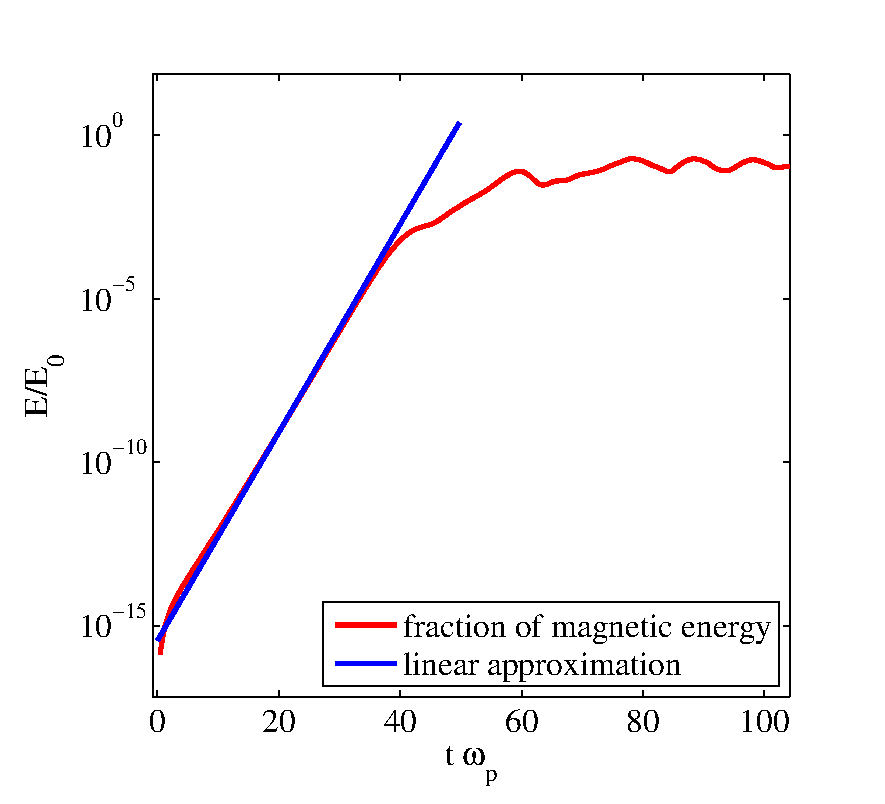
\includegraphics[width=0.99\linewidth]{twostream.eps}}
		\caption{Time dependence of the ratio of the magnetic energy to the full initial energy  in case of the two stream instability.}
		\label{twostream}
	\end{minipage}\hfill
	\begin{minipage}{0.49\textwidth}
		%\center{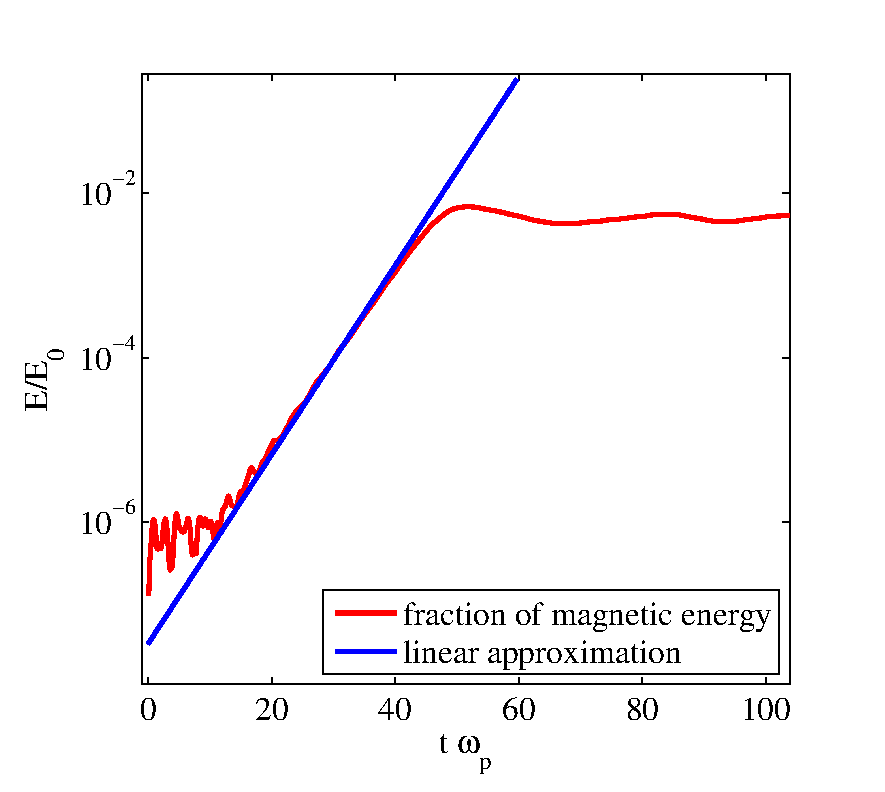
\includegraphics[width=0.99\linewidth]{weibel.eps}}
		\caption{Time dependence of the ratio of the magnetic energy to the full initial energy  in case of the Weibel instability.}
		\label{weibel}
	\end{minipage}
\end{figure}

The second test of the code is the Weibel instability \cite{Weibel1959}, which occurs when the temperature in one spatial direction is smaller then in the other two. This instability has many different cases, we chose the one which was studied by Yoon et al. \cite{Yoon1987}. In this case electrons have delta distribution in transverse momentum and uniform one in parallel. Electron distribution function is:
\begin{equation}
F\left(p_\perp^2, p_\parallel\right)=\frac{1}{2\pi p_{0\perp}}\delta\left(p_\perp - p_{0\perp}\right)\frac{1}{2p_{0\parallel}}H(p_{0\parallel}^2-p_\parallel^2),
\end{equation}
where $\delta$ is the delta-function, $H$ is the Heaviside function, $p_\perp, p_\parallel$ are momentum of particles in perpendicular and parallel directions , respectively, and $p_{0\perp}, p_{0\parallel}$ are constants which determine dispersion of distribution. Dispersion relation for this case can be directly solved, while the expression for the increment is rather cumbersome and will not be presented here for brevity. As shown in Figure \ref{weibel} the numerical simulation with parameters $p_{0\perp} = 20m_e c$ and $p_{0\parallel} = 2 m_e c$ is in good correspondence with the theory.

These results show that our PIC code gives consistent results in the simulation of plasma instabilities and can be applied to more complicated cases.
\section{Shock wave simulation}
We studied the influence of fractions of heavy ions on the shock wave, in particular, the spectrum of particles and the shape of the shock wave. We present results of two simulations with different compositions of the plasma : pure protons and electrons in the first case and with the admixture of alpha particles in the second case. Initially the homogeneous flux is  moving from the right free boundary to the left. On the left side there is a reflecting super-conducting wall, which causes formation of shock wave. Simulations are one-dimensional and have following parameters: initial velocity $v = 0.2c$, number densities $n_e = 10^{-4} \rm{cm}^{-3}$, $n_p = 10^{-4} \rm{cm}^{-3}$ in the first simulation and $n_e = 10^{-4} \rm{cm}^{-3}$, $n_p = 0.6\cdot10^{-4} \rm{cm}^{-3}$, $n_\alpha = 0.2\cdot10^{-4} \rm{cm}^{-3}$ in the second, temperature $5\cdot10^8 \rm{K}$, magnetic field $B_\parallel = 10^{-4} \rm{G}, B_\perp= 0.7\cdot10^{-4} \rm{G}$, the full size of the box $L = 1\cdot10^{12} \rm{cm}$, the number of cells $N=2\cdot10^4$. Electron mass is reduced to $m_e = \frac{m_p}{20}$. The full time of simulation is $T = 2000 {\omega_p}^{-1}$.
\begin{figure}[h!]
	\centering
	\begin{minipage}{0.49\textwidth}
		\centering
		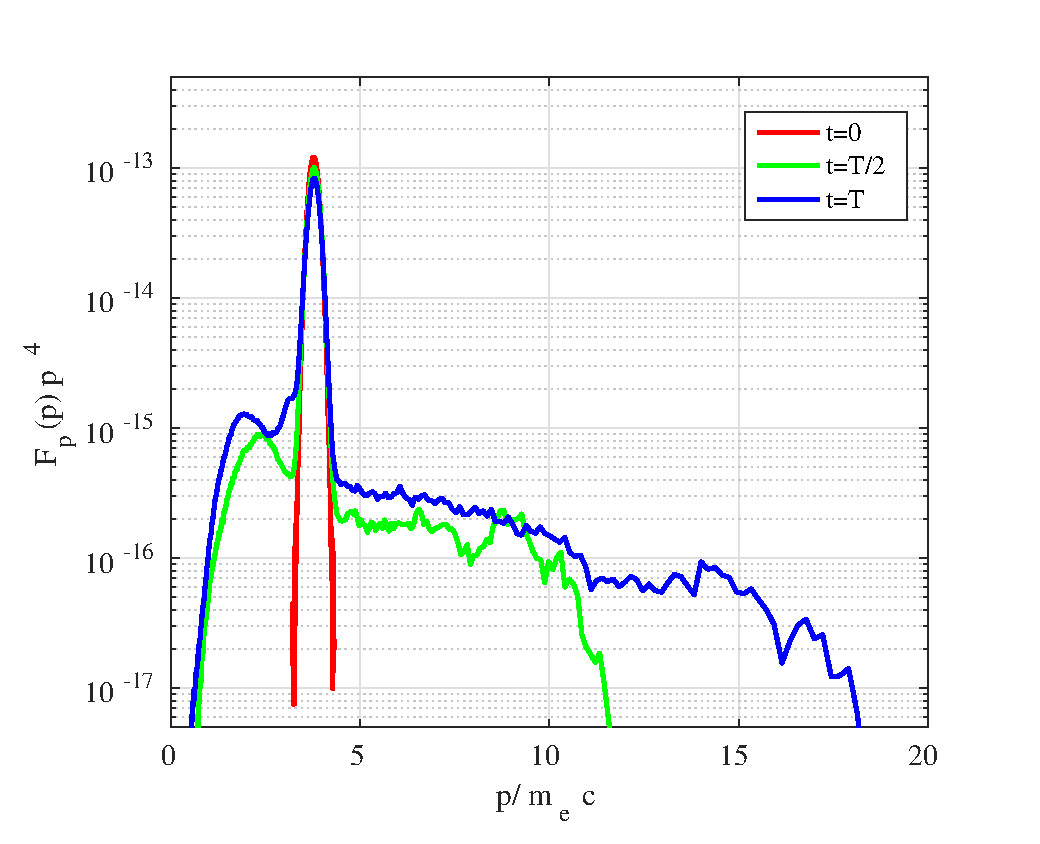
\includegraphics[width=0.98\textwidth]{fig/protons.eps} 
		\caption{Distribution of protons in the simulation without alpha particles.}
		\label{protons}
	\end{minipage}\hfill
	\begin{minipage}{0.49\textwidth}
		\centering
		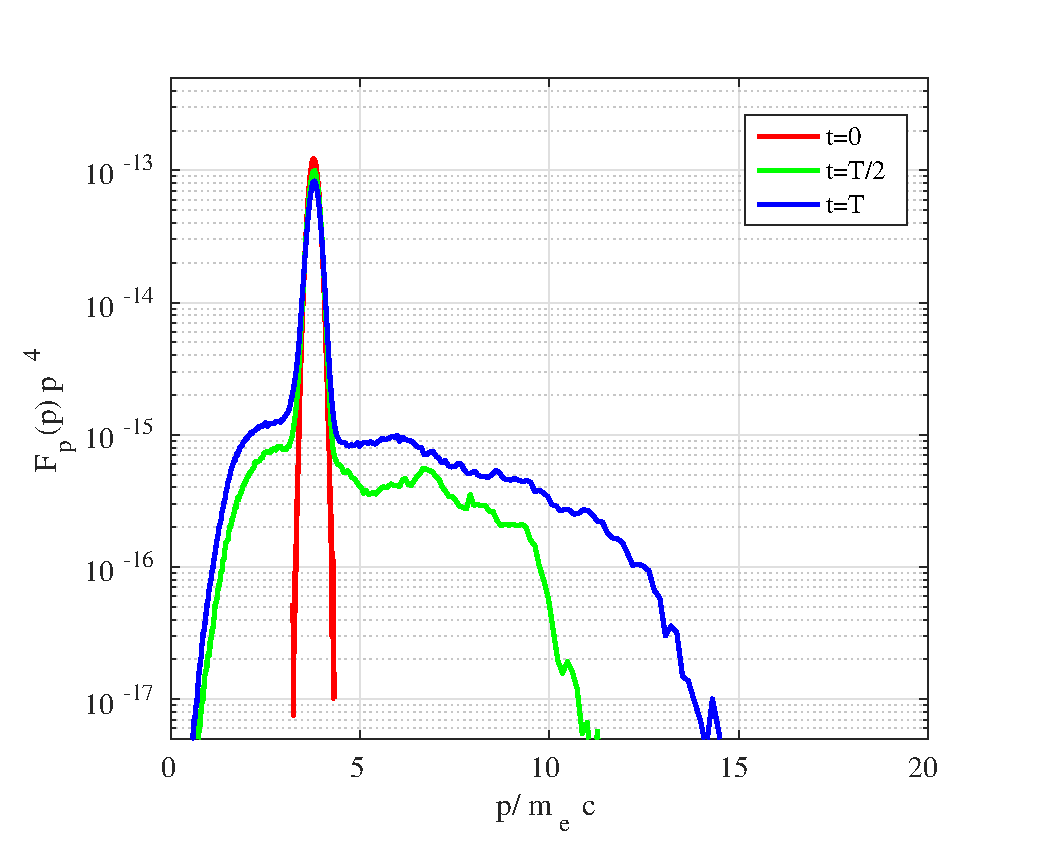
\includegraphics[width=0.98\textwidth]{fig/protons_with_He.eps} 
		\caption{Distribution of protons in the simulation with alpha particles.}
		\label{protons_with_alpha}
	\end{minipage}
\end{figure}
\begin{figure}[h!]
	\centering
	\begin{minipage}{0.49\textwidth}
		\centering
		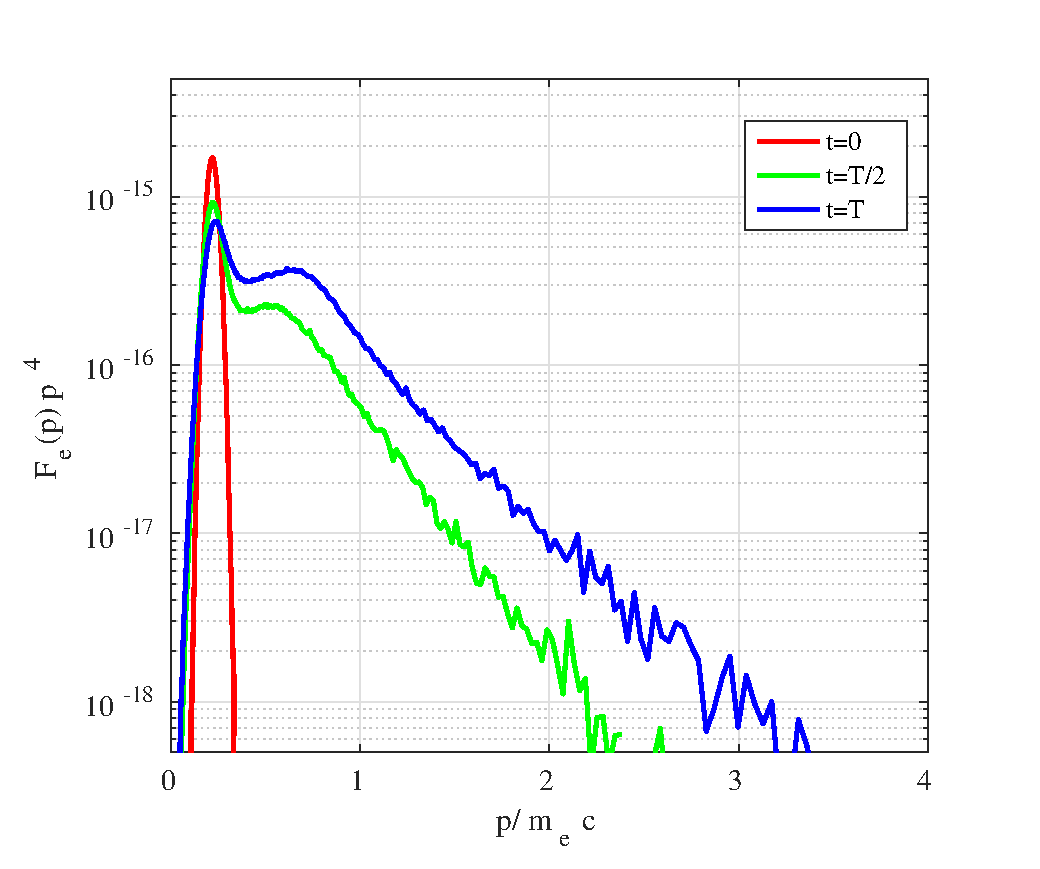
\includegraphics[width=0.98\textwidth]{fig/electrons.eps} 
		\caption{Distribution of electrons in the simulation without alpha particles.}
		\label{electrons}
	\end{minipage}\hfill
	\begin{minipage}{0.49\textwidth}
		\centering
		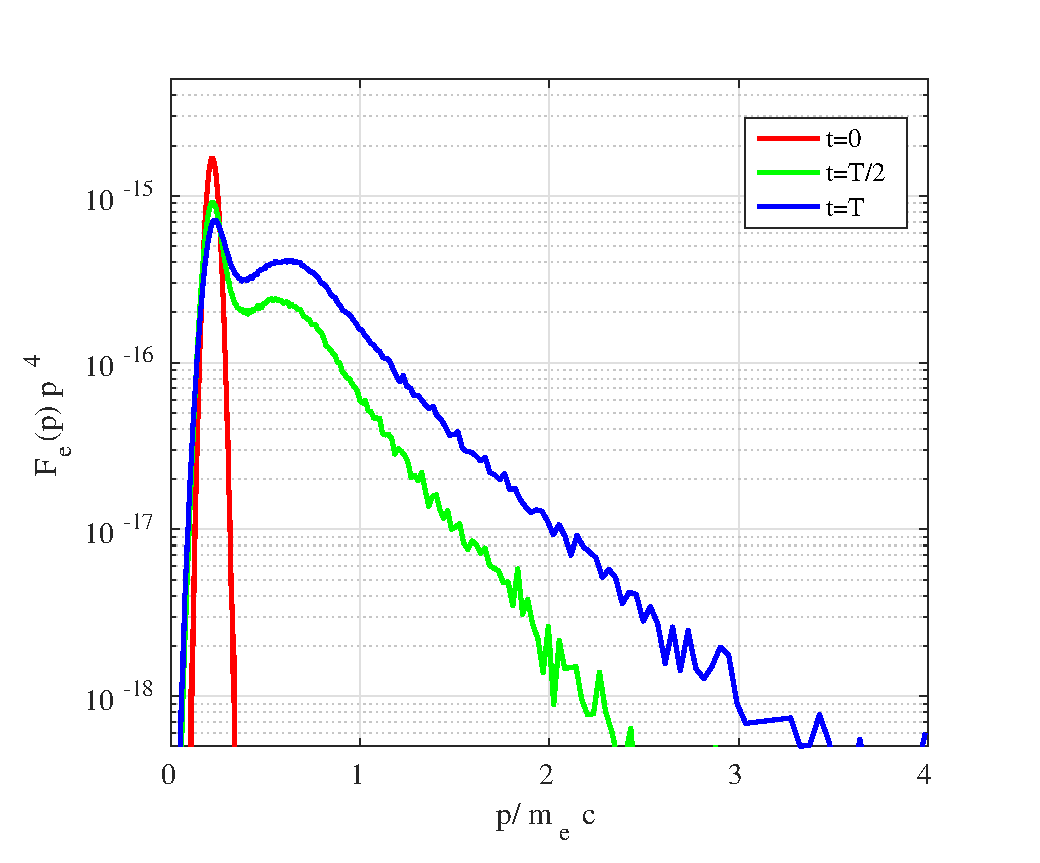
\includegraphics[width=0.98\textwidth]{fig/electrons_with_He.eps} 
		\caption{Distribution of electrons in the simulation with alpha particles.}
		\label{electrons_with_alpha}
	\end{minipage}
\end{figure}

The results presented in Figures \ref{protons}-\ref{electrons_with_alpha} show that the values of $F(p)p^4$ for high energies are much greater for protons, than for electrons in both simulations. Also electrons need much more time to be accelerated and to form spectrum $\propto p^{-4}$. It means that protons are injected into the acceleration process more efficiently, and it is consistent with the work of Park et al. {\cite{Park2015}}. Also we have shown that minority of heavy ions increases the spectrum of protons and do not have influence on the spectrum of electrons. It can be explained by the fact, that heavy ions form the large scale turbulence and protons can efficiently scatter on this turbulence. Otherwise for electrons turbulence produced by protons is already enough large-scale  and the influence of heavy ions is neglectable. 

\section{Conclusions}
In this paper we presented the developed 3D implicit particle-in-cell code, which can be applied for various problems in the collisionless plasma. We have tested it and obtained results, that are consistent with theoretical predictions. We studied the influence of admixture of heavy ions on the evolution of the shock wave and simulations have shown that the presence of heavy ions increases the number of accelerated particles. Further research is necessary in order to study this phenomena in detail.
\ack
A M Bykov, P E  Gladilin and S M  Osipov have developed the implicit fields solver module, which provides conservation of the divergenceless magnetic field. 
V I Romansky acknowledges support from RSF grant 16-12-10519 which was used to develop the
particle mover, parallelization and perform the testing of the code.


The results of the work were obtained using computational resources of Peter the Great Saint-Petersburg Polytechnic University Supercomputing Center (http://www.spbstu.ru).
\section*{References}
\begin{thebibliography}{20}
\bibitem{Bell1978} Bell A R 1978 \textit{MNRAS} \textbf{182} 147
\bibitem{Blandford1978} Blandford R D and Ostriker J P 1978 \textit{Astrophys. J.} \textbf{221} L29 
\bibitem{Berezhko2003} Berezhko E G, Ksenofontov L T and V{\"o}lk H J  2003 \textit{A}{\&}\textit{A} \textbf{412} L11
\bibitem{Uchiyama2007} Uchiyama Y, Aharonian F A, Tanaka T, Takahashi T and Maeda Y 2007 \textit{Nature} \textbf{449} 576
\bibitem{Lapenta2006} Lapenta G, Brackbill J U and Ricci P 2006 \textit{Phys. Plasmas} \textbf{13} 055904
\bibitem{Noguchi2007} Noguchi K, Tronci C, Zuccaro G and Lapenta G 2007 \textit{Phys. Plasmas} \textbf{14} 042308
\bibitem{Weibel1959} Weibel E S 1959 \textit{Phys. Rev. Lett.} \textbf{2} 83
\bibitem{Yoon1987} Yoon P H and Davidson R C 1987 \textit{Phys. Rev. A} \textbf{35} 2718
\bibitem{Park2015} Park J, Caprioli D and Spitkovsky A 2015 \textit{Phys. Rev. Lett.} \textbf{114} 085003
\end{thebibliography}
\end{document}